\subsubsection{Description}
Our \gls{glvs} Accumulator is made using 18650 Li-ion cells Sony VTC-5. The configuration is 6s1p which equals to our low-voltage system voltage 24 V. Datasheet is in appendix.

\subsubsection{Wiring, cables, current calculations, connectors}
%Describe wiring, show schematics, describe connectors and cables and show useful data regarding the wiring.  Include information on the working voltage and current rating of the accumulator.

The \gls{glvs} Accumulator is made of 18650 cells. They are held together by modular structure and interconnected by nickel tabs using spot welding. On each end, there is small tab spot welded to the cell and main wire soldered on the tab. On the other end of the mains wire (positive and negative), there is a XT-60 connector soldered. Balancing wires are soldered to the respective interconnecting tabs. The battery use 7-pin balancing connector JST-XH, so that the whole accumulator is using standards widely used in RC models. The intent is to have the ability to use wide range of diagnostic tool or chargers made to this standard.

The battery also have 4 \glspl{ntc} for measuring cells temperature connected by separate connector.

The peak discharge rating of the cells is 30 A, the XT-60 connector continuous current rating is 60A. The corresponding input in \gls{ecub} where the accumulator is connected is fused by 20 A main fuse. The wire used for mains between the cells and XT-60 connector is silicone insulated copper cable of cross-section 2,5 mm$^2$ which gives ampacity of 30 A, well above the fuse.

The balancing wires are AWG22 with ampacity 5 A and each is fused with 2 A SMD fuse at the \gls{pcb} behind the JST-XH connector.

\begin{table}[H]
	\centering
	\caption{GLVS accumualtor general parameters.}
	\begin{tabu}{|X|X|}\hline
		Cell/Accumulator: & Sony VTC-5 18650 Li-ion\\\hline
		Accumulator configuration – parallel: & 1 \\\hline
		Accumulator configuration – series: & 6 \\\hline
		Maximum Voltage: & 25.2 V \\\hline
		Nominal Voltage: & 21.6 V \\\hline
		Minimum Voltage: & 12 V \\\hline
		Max. Continuous Discharge Current: & 20 A \\\hline
		Peak Discharge Current: & 30 A \\\hline
		Peak Discharge Current Time: & Till temp rise to 80 $^\circ$C (refer to \hyperref[app:sony-vtc5]{datasheet}, section 2.8.2) \\\hline
		Max. Continuous Charge Current & 4 A\\\hline
		Total capacity[MJ]: & 0.194 MJ \\\hline
	\end{tabu}%
	\label{tab:LVbatt-general}%
\end{table}%

GLVS cell datasheet: \ref{app:sony-vtc5}

\subsubsection{Position in car}
Positon of whole ECUB can be seen here \ref{fig:ecub_position}.
\begin{figure}[H]
	\centering
	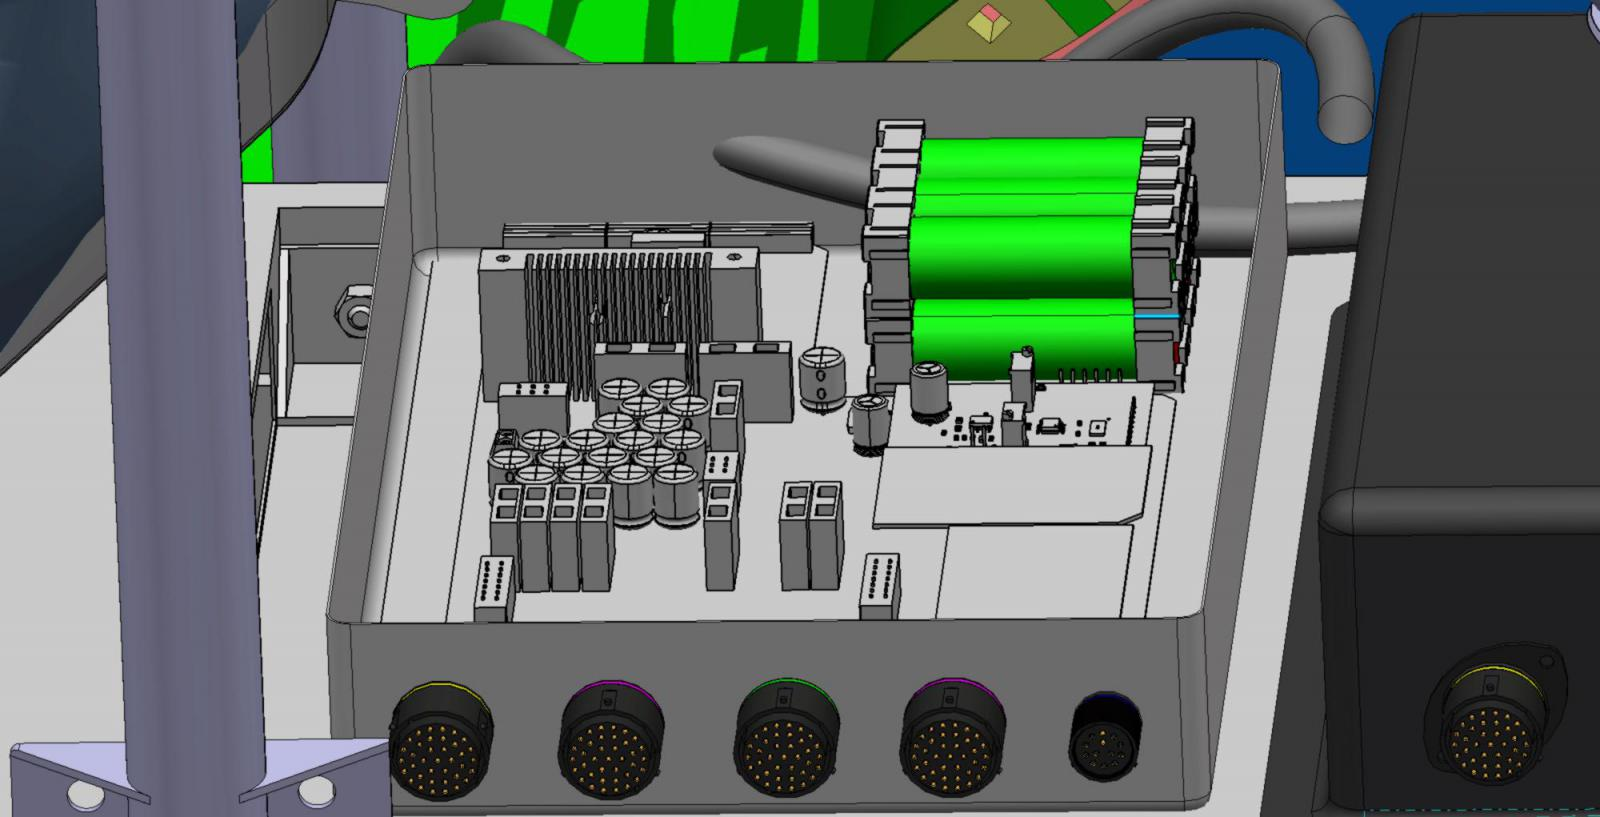
\includegraphics[width=\textwidth,clip]{./img/ECUB_BATTERY_POSITION.jpg}
	\caption{\gls{glvs} battery position.}
	\label{fig:GLVS_battery_position}
\end{figure}